% ----- Consignes exo 1 ----- %
\begin{td-exo}[Problème du \textsc{Feedback Vertex Set}]\,\\ % 1 
	Le problème du \textsc{Feedback Vertex Set} défini ci-dessous est un problème fondamental en base de données.
    Dans les systèmes d'exploitation, ce problème joue un rôle important dans l'étude de la récupération de données après des crashs ou des blocages.
    Dans le graphe des processus d'un système d'exploitation, chaque cycle dirigé correspond à une situation d'impasse.
    Afin de résoudre toutes les impasses, certains processus bloqués doivent être abandonnés.
    Un \textsc{Feedback Vertex Set} dans le graphe correspond à un nombre minimum de processus qu'il faut abandonner.
	
    \vspace{-6mm}
\begin{algorithm}[H]
    \caption{\textsc{Feedback Vertex Set}}
    \begin{algorithmic}
        \Require{Soit \(G = (V, E)\) un graphe orienté et \(k\in \bb N\)}
        \Ensure{Existe-t-il un ensemble \(S \subset V\) de \(k\) sommets tel que \(G \setminus S\) est un graphe sans circuit (tous les arcs sont orientés dans le même sens)?}
    \end{algorithmic}
\end{algorithm}

    On considère les figures ci-dessous:

    \begin{center}
        \begin{minipage}{0.48\linewidth}
            \centering
            \ffigbox[\FBwidth]{%
\caption{\centering Exemple pour le \textsc{Feedback Vertex Set}}\label{fig:dm1_ex01_f2}
}{
    \fbox{
        \begin{tikzpicture}[scale=1, main node/.style={circle, draw, fill=blue!20, inner sep=1pt, font=\scriptsize, minimum size=6mm, text=black}]
            % les sommets initiaux
            \node[main node] (a) at (0,0) {\(a\)};
            \node[main node] (b) at (2, 0) {\(b\)};
            \node[main node] (c) at (2,-2) {\(c\)};
            \node[main node] (d) at (0,-2) {\(d\)};
            \node[main node] (e) at (-2,-4) {\(e\)};

            % les arcs avec capacités
            \draw[-{Stealth}] (a) edge[bend left] (b);
            \draw[-{Stealth}] (b) edge[bend left] (a);
            \draw[-{Stealth}] (a) edge[bend left] (d);
            \draw[-{Stealth}] (d) edge[bend left] (a);
            \draw[-{Stealth}] (b) edge[bend left] (c);
            \draw[-{Stealth}] (c) edge[bend left] (b);
            \draw[-{Stealth}] (c) edge[bend left] (d);
            \draw[-{Stealth}] (d) edge[bend left] (c);
            \draw[-{Stealth}] (d) edge[bend left] (e);
            \draw[-{Stealth}] (e) edge[bend left] (d);

        \end{tikzpicture}
    }
}
        \end{minipage}\hfill
        \begin{minipage}{0.48\linewidth}
            \centering
            \ffigbox[\FBwidth]{%
\caption{\centering Instance initiale pour le \textsc{Vertex Cover}}\label{fig:dm1_ex01_f3}
}{
    \fbox{
        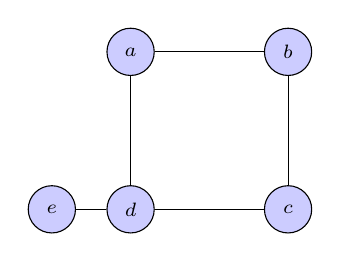
\begin{tikzpicture}[scale=1, main node/.style={circle, draw, fill=blue!20, inner sep=1pt, font=\scriptsize, minimum size=6mm, text=black}]
            % les sommets initiaux
            \node[main node] (a) at (0,0) {\(a\)};
            \node[main node] (b) at (2, 0) {\(b\)};
            \node[main node] (c) at (2,-2) {\(c\)};
            \node[main node] (d) at (0,-2) {\(d\)};
            \node[main node] (e) at (-1,-2) {\(e\)};

            % les arcs avec capacités
            \draw (a) edge (b);
            \draw (b) edge (c);
            \draw (c) edge (d);
            \draw (d) edge (a);
            \draw (d) edge (e);
            
        \end{tikzpicture}
    }
}
        \end{minipage}
    \end{center}

    \begin{enumerate}
        \item Donner l'ensemble \(S\) pour le graphe orienté donné par la figure~\ref{fig:dm1_ex01_f2}.
        \item Proposer une réduction à partir de \textsc{Vertex Cover} et effectuer la preuve de NP-complétude.
        \item Appliquer votre réduction sur le graphe donné par la figure~\ref{fig:dm1_ex01_f3}.
    \end{enumerate}
\end{td-exo}

% ----- Solutions exo 1 ----- %
\iftoggle{showsolutions}{ 
	\begin{td-sol}[]\ % 1
		\begin{enumerate}
            \item On commence par essayer de trouver un ensemble \(S\) de taille \(k = 1\).
            Si on retire \(e\) ou \(d\) alors le cycle \(a-b\) subsiste.
            Sinon c'est le cycle \(e-d\) qui subsiste.
            Il n'y a donc pas de solution pour \(k = 1\).
            On cherche maintenant une solution pour \(k=2\).
            Il faut casser chaque cycle dans le graphe donc il faut pour chaque paire de sommets adjacents dans le graphe, retirer un des deux sommets.
            Si on choisit \(S = \{b, d\}\) il n'y a plus de cycles dans le graphe \(G \setminus S = \{a, c, e\}\).
            Alors \(S = \{b, d\}\) est bien solution minimale du problème avec \(k=2\).

            \item Commencons par montrer que le problème de \textsc{Feedback Vertex Set} appartient à la classe NP.\@
            Soit \(S\) une solution au problème de \textsc{Feedback Vertex Set}.
            On commence par vérifier que \(S\) est bien de taille \(k\) (se fait en temps linéaire).
            Ensuite, pour vérifier la validité d'une telle solution, on retire \(S\) du graphe \(G\) (se fait en temps linéaire) puis on effectue un BFS sur chaque sommet de \(G\) (polynomial en le nombre de sommets) pour vérifier qu'on ne retombe pas sur le sommet de départ.
            Ainsi le problème de \textsc{Feedback Vertex Set} est bien NP.\@

            Montrons maintenant qu'on peut réduire le problème de \textsc{Vertex Cover} à un problème de \textsc{Feedback Vertex Set}.
            Soit \(G = (V, E)\) un graphe non orienté. 
            On construit le graphe \(G' = (V', E')\) comme suit: pour chaque sommet \(v\in V\) de \(G\), on rajoute \(v' = v \in V'\).
            Pour chaque arête \({u, v}\in E\), on rajoute deux arcs orientés \({u, v},{v, u}\) dans \(E'\).
            Alors \(G' = (V', E')\) correspond au graphe \(G\) où chaque arête est remplacée par deux arcs de sens opposé.
            Cette construction peut se faire en temps polynomial.

            On commence par montrer le sens direct.
            Soit \(S\) une solution au \textsc{Vertex Cover} dans \(G\).
            Alors, toute arête \({u, v}\in E\) a bien \(u\in S\) ou \(v\in S\).
            Alors, tous les 2-cycles dans \(G'\) sont cassés (sinon l'arête correspondante ne serait pas couverte par \(S\)).
            Alors tous les sommets de \(G'\) sont isolés et \(G'\) n'a donc aucun cycle.
            On a trouvé une solution à \textsc{Feedback Vertex Set} dans \(G'\) à partir d'une solution de \textsc{Vertex Cover} dans \(G\).

            Maintenant le sens indirect.
            Soit \(S\) une solution de \textsc{Feedback Vertex Set} dans \(G'\).
            Alors, toute arête \({u, v}\in E'\) a bien \(u\in S\) ou \(v\in S\) (sinon \(u-v-u\) formerait un cycle).
            Alors, toutes les arêtes dans \(E\) sont bien couvertes par \(S\) dans \(G\) (sinon on aurait un 2-cycle induit dans \(G'\)).
            On a trouvé une solution à \textsc{Vertex Cover} dans \(G\) à partir d'une solution de \textsc{Feedback Vertex Set} dans \(G'\).

            Alors, le problème de \textsc{Feedback Vertex Set} est NP-complet.

            \item Appliquons la réduction au graphe~\ref{fig:dm1_ex01_f4}.

            On commence par créer le graphe \(G'\) comme décrit dans la réduction:

            \vspace{9px}
            \ffigbox[\FBwidth]{%
\caption{\centering Graphe \(G'\) obtenu par réduction}\label{fig:dm1_ex01_f4}
}{
    \fbox{
        \begin{tikzpicture}[scale=1, main node/.style={circle, draw, fill=blue!20, inner sep=1pt, font=\scriptsize, minimum size=6mm, text=black}]
            % les sommets initiaux
            \node[main node] (a) at (0,0) {\(a\)};
            \node[main node] (b) at (2, 0) {\(b\)};
            \node[main node] (c) at (2,-2) {\(c\)};
            \node[main node] (d) at (0,-2) {\(d\)};
            \node[main node] (e) at (-1,-2) {\(e\)};

            % les arcs avec capacités
            \draw[-{Stealth}] (a) edge[bend left] (b);
            \draw[-{Stealth}] (b) edge[bend left] (c);
            \draw[-{Stealth}] (c) edge[bend left] (d);
            \draw[-{Stealth}] (d) edge[bend left] (a);
            \draw[-{Stealth}] (d) edge[bend left] (e);

            \draw[-{Stealth}] (b) edge[bend left] (a);
            \draw[-{Stealth}] (c) edge[bend left] (b);
            \draw[-{Stealth}] (d) edge[bend left] (c);
            \draw[-{Stealth}] (a) edge[bend left] (d);
            \draw[-{Stealth}] (e) edge[bend left] (d);
            
        \end{tikzpicture}
    }
}

            Une solution au problème de \textsc{Vertex Cover} dans le graphe de départ est \(S = \{d, b\}\).
            Si on retire \(S\) au graphe \(G'\) on obtient:
            \begin{center}
                \begin{minipage}{0.48\linewidth}
                    \centering
                    \ffigbox[\FBwidth]{%
\caption{\centering Graphe \(G'\) obtenu par réduction}\label{fig:dm1_ex01_f5}
}{
    \fbox{
        \begin{tikzpicture}[scale=1, main node/.style={circle, draw, fill=blue!20, inner sep=1pt, font=\scriptsize, minimum size=6mm, text=black}]
            % les sommets initiaux
            \node[main node] (a) at (0,0) {\(a\)};
            \node[main node, draw=gray, fill=gray!10, path picture={
                \draw[gray, line width=0.6pt]
                (path picture bounding box.south west) --
                (path picture bounding box.north east);
                \draw[gray, line width=0.6pt]
                (path picture bounding box.north west) --
                (path picture bounding box.south east);
            }] (b) at (2,0) {\(b\)};
            \node[main node] (c) at (2,-2) {\(c\)};
            \node[main node, draw=gray, fill=gray!10, path picture={
                \draw[gray, line width=0.6pt]
                (path picture bounding box.south west) --
                (path picture bounding box.north east);
                \draw[gray, line width=0.6pt]
                (path picture bounding box.north west) --
                (path picture bounding box.south east);
            }] (d) at (0,-2) {\(d\)};
            \node[main node] (e) at (-1,-2) {\(e\)};

            % les arcs avec capacités 
            \draw[-{Stealth}, dashed, gray!10!pagetext] (a) edge[bend left] (b);
            \draw[-{Stealth}, dashed, gray!10!pagetext] (b) edge[bend left] (c);
            \draw[-{Stealth}, dashed, gray!10!pagetext] (c) edge[bend left] (d);
            \draw[-{Stealth}, dashed, gray!10!pagetext] (d) edge[bend left] (a);
            \draw[-{Stealth}, dashed, gray!10!pagetext] (d) edge[bend left] (e);

            \draw[-{Stealth}, dashed, gray!10!pagetext] (b) edge[bend left] (a);
            \draw[-{Stealth}, dashed, gray!10!pagetext] (c) edge[bend left] (b);
            \draw[-{Stealth}, dashed, gray!10!pagetext] (d) edge[bend left] (c);
            \draw[-{Stealth}, dashed, gray!10!pagetext] (a) edge[bend left] (d);
            \draw[-{Stealth}, dashed, gray!10!pagetext] (e) edge[bend left] (d);
            
        \end{tikzpicture}
    }
}
                \end{minipage}\hfill
                \begin{minipage}{0.48\linewidth}
                    \centering
                    \ffigbox[\FBwidth]{%
\caption{\centering Graphe \(G'\) simplifié}\label{fig:dm1_ex01_f6}
}{
    \fbox{
        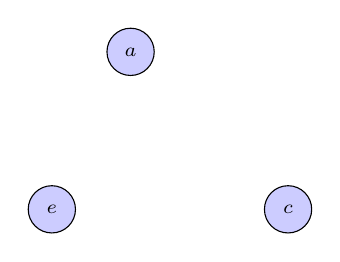
\begin{tikzpicture}[scale=1, main node/.style={circle, draw, fill=blue!20, inner sep=1pt, font=\scriptsize, minimum size=6mm, text=black}]
            % les sommets initiaux
            \node[main node] (a) at (0,0) {\(a\)};
            \node[main node] (c) at (2,-2) {\(c\)};
            \node[main node] (e) at (-1,-2) {\(e\)};
        \end{tikzpicture}
    }
}
                \end{minipage}
            \end{center}
        \end{enumerate}
	\end{td-sol}
}{}